\chapter{Toepassingen van diepte-eerst zoeken}
\begin{itemize}
	\item Notatie:
	\begin{itemize}
		\item Het aantal knopen is $n$.
		\item Het aantal verbindingen is $m$.
	\end{itemize}
\end{itemize}
\section{Enkelvoudige samenhang van grafen}
\subsection{Samenhangende componenten van een ongerichte graaf}
\begin{itemize}
	\item Een \textbf{samenhangende ongerichte graaf} is een graaf waarbij er een weg bestaat tussen elk paar knopen.
	\item Een \textbf{niet samenhangende ongerichte graaf} bestaat dan uit zo groot mogelijke samenhangende componenten.
	\item Diepte-eerst zoeken vindt alle knopen die met wortel van de diepte-eerst boom verbonden zijn.
	\begin{itemize}
		\item Een ongerichte graaf is samenhangend wanneer die boom alle knopen bevat.
		\item Als er meerdere bomen zijn, vormen deze de samenhangende componenten.
		\item Diepte-eerst zoeken is $\Theta(n + m)$.
	\end{itemize}
\end{itemize}

\subsection{Sterk samenhangende componenten van een gerichte graaf}
\begin{itemize}
	\item Een \textbf{sterk samenhangende gerichte graaf} is een graaf waarbij er een weg tussen elk paar knopen in beide richtingen (niet perse dezelfde verbindingen) bestaat (cfr. figuur \ref{fig:sterk_samenhangende_graaf}).
	\begin{figure}[ht]
		\centering
		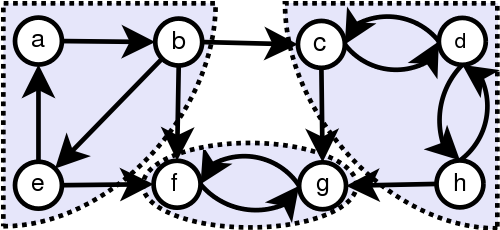
\includegraphics[width=0.5\textwidth]{img/sterk_samenhangende_graaf}
		\caption{Een sterk samenhangende graaf.}
		\label{fig:sterk_samenhangende_graaf}
	\end{figure}
				
	\item Een \textbf{zwak samenhangende gerichte graaf} is een graaf die niet sterk, maar toch samenhangend is indien de richtingen buiten beschouwing gelaten worden. Een graaf die niet sterk samenhangend is, bestaat uit zo groot mogelijke sterk samenhangende componenten. 
	\item Sommige algoritmen gaan ervan uit de een graaf sterk samenhangend is. Men moet dus eerst deze componenten bepalen, meestal via een \textbf{componentengraaf} die:
	\begin{itemize}
		\item een knoop heeft voor elk sterk samenhangend component,
		\item en een verbinding van knoop $a$ naar knoop $b$ indien er in de originele graaf een verbinding van één van de knopen van $a$ naar één van de knopen van $b$ is. 
	\end{itemize}
	\item De componentgraaf bevat geen lussen, anders wil dit zeggen dat die knoop zelf nog opgesplitst zou kunnen worden in twee sterk samenhangende componenten.
	\item De sterk samenhangende componenten \textbf{in een gerichte graaf} kunnen bekomen worden met behulp van diepte-eerst zoeken (Kosaraju's Algorithm):
	\begin{enumerate}
		\item Stel de omgekeerde graaf op, door de richting van elke verbinding om te keren.
		\item Pas diepte-eerst zoeken toe op deze omgekeerde graaf, waarbij de knopen in postorder genummered worden.
		\item Pas diepte-eerst zoeken toe op de originele graaf, met als startknoop steeds de resterende knoop met het hoogste postordernummer. Het resultaat is een diepte-eerst bos, waarvan de bomen sterk samenhangende componenten zijn.
	\end{enumerate}
	\item We willen aantonen dat de wortel van elke boom in beide richtingen verbonden is met elk van zijn knopen.  Op die manier is elke andere knoop in beide richtingen verbonden door de wortel en klopt het algoritme.
	\begin{itemize}
		\item Via de boomtakken is er een weg van de wortel $w$ naar elk van de knopen $u$ in de boom. 
		\item Er is dan ook een weg van $u$ naar $w$ in de omgekeerde graaf.
		\item De wortel $w$ is altijd een voorouder van $u$ in een diepte-eerst boom van de omgekeerde graaf.
		item 
		\item Hieruit volgt dat er een weg van $w$ naar $u$ bestaat in de omgekeerde graaf.
		\item Er is dan ook een weg van $u$ naar $w$ in de originele graaf.
	\end{itemize}

	\item Diepte-eerst zoeken is $\Theta(n + m)$ voor ijle en $\Theta(n^2)$ voor dichte grafen. Het omkeren van de graaf is ook $\Theta(n + m)$ voor ijle en $\Theta(n^2)$ voor dichte grafen.
\end{itemize}




\section{Dubbele samenhang van ongerichte grafen}
Twee definities:
\begin{itemize}
	\item \textbf{Brug.} Een brug is een verbinding dat, indien deze wordt weggenomen, de graaf in twee deelgrafen opsplitst. Een graaf zonder bruggen noemt men \textbf{dubbel lijnsamenhangend}; als er tussen elk paar knopen minstens twee onafhankelijke wegen bestaan, dan is een graaf zeker dubbel lijnsamenhangend.
	\item \textbf{Scharnierpunt.} Een scharnierpunt is een knoop dat, indien deze wordt weggenomen, de graaf in ten minste twee deelgrafen opsplitst. Een graaf zonder scharnierpunten noemt men \textbf{dubbel knoopsamenhangend} (of dubbel samenhangend). Een graaf met scharnierpunten kan onderverdeeld worden in dubbel knoopsamenhangende componenten. Als er tussen elk paar knopen twee onafhankelijke wegen bestaan, dan is de graaf dubbel knoopsamenhangend.
\end{itemize}

Scharnierpunten, dubbel knoopsamenhangende componenten, bruggen en dubbel lijnsamenhangende componenten kunnen opnieuw via diepte-eerst zoeken gevonden worden:
\begin{enumerate}
	\item Stel de diepte-eerst boom op, waarbij de knopen in preorder genummerd worden. 
	\item Bepaal voor elke knoop $u$ de laagst genummerde knoop die vanuit $u$ kan bereikt worden via een weg bestaande uit nul of meer dalende boomtakken gevolgd door één terugverbinding. 
	\item Indien alle kinderen van een knoop op die manier een knoop kunnen bereiken die hoger in de boom ligt dan hemzelf, dan is de knoop zeker niet samenhangend. De wortel is een scharnierpunt indien hij meer dan één kind in heeft. \todo{hoe bruggen vinden?}
\end{enumerate}
Diepte-eerst zoeken is $\Theta(n + m)$ voor ijle en $\Theta(n^2)$ voor dichte grafen.
\section{Eulercircuit}
Een eulercircuit is een \textbf{gesloten pad} in een graaf die alle \textbf{verbindingen} éénmaal bevat. 
\subsection{Ongerichte grafen}

\begin{figure}[ht]
\centering
\begin{subfigure}{.5\textwidth}
	\centering
	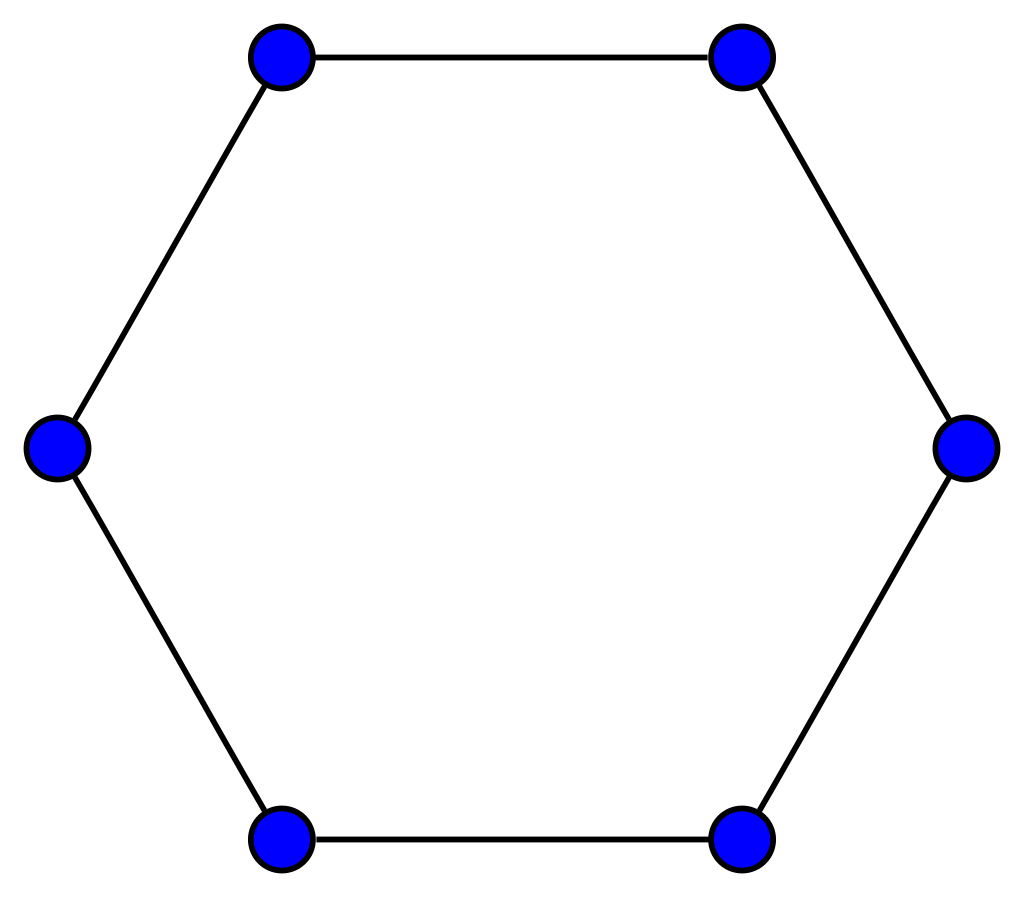
\includegraphics[width=.4\linewidth]{eulergraph_simple}
	\caption{Een Eulegraaf met 6 knopen en 6 verbindingen.}
	\label{fig:eulergraph_simple}
  \end{subfigure}%
  \begin{subfigure}{.5\textwidth}
	\centering
	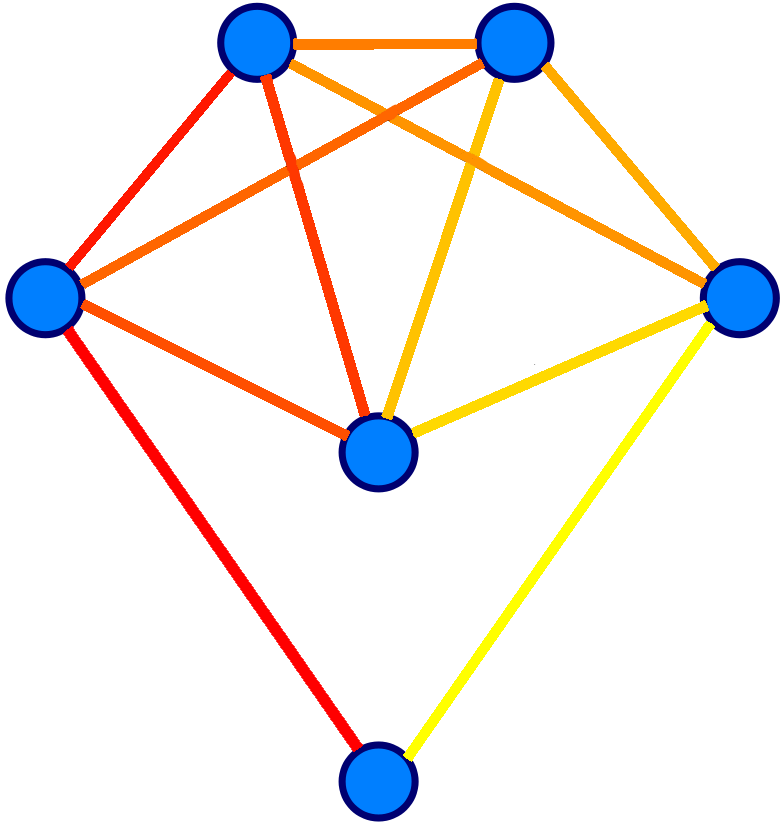
\includegraphics[width=.4\linewidth]{eulergraph_complex}
	\caption{Een Eulergraaf waarbij de volgorde van de verbindingen die het Eulercircuit opmaken gekleurd worden van rood naar geel.}
	\label{fig:eulergraph_complex}
  \end{subfigure}
\end{figure}

\begin{itemize}
	\item Een Eulergraaf is een graaf met een eulercircuit. 
	\item Volgende eigenschappen zijn equivalent.
	\begin{enumerate}
		\item Een samenhangende graaf $G$ is een Eulergraaf.
		\begin{itemize}
			\item Dit volgt uit de derde eigenschap.
			\item Stel dat $L$ één van de lussen van $G$ is.
			\item Als $L$ een Eulercircuit is dan is $G$ een Eulergraaf.
			\item Zoniet bestaat er een andere lus $L'$ die een gemeenschappelijke knoop $k$ heeft met $L$.
			\item Aangezien elke verbinding tot één lus behoort, kunnen deze twee lussen bij knoop $k$ samengevoegd worden.
			\item Uiteindelijk bekomen we een Eulercircuit.
		\end{itemize}
		\item De graad van elke knoop van $G$ is even.
		\begin{itemize}
			\item Dit volgt uit de eerste eigenschap.
			\item Als een knoop $k$ voorkomt op een Eulercircuit, draagt dat twee bij tot zijn graad.
			\begin{itemize}
				\item Er is een verbinding nodig om de knoop te bereiken, en ook een verbinding om de knoop te verlaten.
			\end{itemize}
		\end{itemize}
		\item De verbindingen van $G$ kunnen onderverdeeld worden in lussen, waarbij elke verbinding slechts behoort tot één enkel lus.
		\begin{itemize}
			\item Dit volgt uit de tweede eigenschap.
			\item Stel dat er $n$ knopen zijn.
			\item Er zijn minstens $n$ verbindingen (want moet terug in startknoop eindigen).
			\begin{itemize}
				\item Eenvoudigste Eulergraaf is een cyclusgraaf (cfr. Figuur \ref{fig:eulergraph_simple}).
			\end{itemize}
			\item $G$ bevat dan minstens één lus.
			\item Als de lus verwijdert wordt, blijft er een niet noodzakelijke samenhangende graaf $H$ over waarvan alle knoopgraden nog steeds even zijn.
			\item Elk van de samenhangende componenten van $H$ kan opnieuw in lussen onderverdeeld worden.
		\end{itemize}
	\end{enumerate}
	\begin{itemize}
		\item Het \textbf{algoritme van Hierholzer} geeft een Eulercircuit voor een Eulergraaf.
		\begin{itemize}
			\item De eerste lus $L$ begint bij een willekeurige knoop. Er worden willekeurig verbindingen gekozen tot dat de knoop opnieuw bereikt wordt.
			\item De volgende lus $L'$ begint bij één van de knopen van $L$ waarvan nog niet alle verbindingen doorlopen zijn. Opnieuw worden willekeurig verbindingen gekozen tot de knoop opnieuw bereikt wordt.
			\item Er worden lussen gegenereerd zolang niet alle verbindingen van een knoop opgebruikt zijn.
		\end{itemize}
	\end{itemize}
\end{itemize}



\subsection{Gerichte grafen}
\begin{itemize}
	\item Een Eulercircuit in een gerichte graaf is slechts mogelijk als de graaf een sterk samenhangende Eulergraaf is.
	\item De constructie verloopt analoog aan de ongerichte Eulergraaf.
\end{itemize}